\documentclass[helvetica,english,nologo,notitle,totpages]{europecv2013}
\usepackage[T1]{fontenc}
\usepackage{graphicx}
\usepackage[a4paper,top=1.27cm,left=1cm,right=1cm,bottom=2cm]{geometry}
\usepackage[english]{babel}
\usepackage{bibentry}
\usepackage{natbib}
\usepackage[ddmmyyyy]{datetime}

\renewcommand{\ttdefault}{phv} % Uses Helvetica instead of fixed width font

%\ecvname{Banescu, Sebastian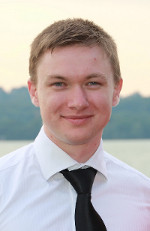
\includegraphics{photo.jpg}}
\ecvname{Sebastian Banescu}
\ecvfootername{Sebastian Banescu \quad Date:~\today}
\ecvaddress{Hochbr\"{u}cker Weg 2, 85396 Eching, Germany}
\ecvtelephone{(+49) 176 4152 5239}
\ecvemail{banescusebi@gmail.com}
%\ecvhomepage{\href{https://www22.in.tum.de/banescu}{www22.in.tum.de/banescu}}
\ecvlinkedin{\href{https://de.linkedin.com/in/sebastianbanescu}{de.linkedin.com/in/sebastianbanescu}}
%\ecvdateofbirth{20 October 1987}
%\ecvgender{Male}
\ecvpicture[width=1.5cm]{photo.jpg}
%\ecvfootnote{For more information go to \url{http://europass.cedefop.eu.int}\\
%\textcopyright~European Communities, 2003.}

\begin{document}
\selectlanguage{english}

\begin{europecv}
\ecvpersonalinfo[10pt]
%\ecvitem{\large\textbf{Desired employment/ Occupational~field}}{\large\textbf{}}

\ecvsection{Education and Training}
\ecvitem{Dates}{October 2014 - April 2017}
\ecvitem{Title of qualification awarded}{\textbf{Dr.~rer.~nat.} \textit{``summa cum laude''}}
\ecvitem{Name of organization}{\textbf{Technical University of Munich, Germany}, Center for Doctoral Studies in Informatics and its Applications (CeDoSIA) Graduate School, Faculty of Informatics}
\ecvitem{PhD Thesis Title}{Characterizing the Strength of Software Obfuscation Against Automated Attacks}
\ecvitem{}{}
\ecvitem{Dates}{September 2010 - August 2012}
\ecvitem{Title of qualification awarded}{\textbf{MSc.Information Security Technologies} \textit{``cum laude''} (GPA: 8.5 of 10, Thesis: 9 of 10)}
%\ecvitem{Principal subjects/Occupational skills covered}{Theoretical and technical expertise in the area of digital communication in general and in information security technology in particular.}
\ecvitem{Scholarship}{Talent Scholarship Program, currently Amandus H. Lundqvist Scholarship Program}
\ecvitem{Name of organization}{\textbf{Technical University of Eindhoven, The Netherlands}, Faculty of Computer Science}
\ecvitem{MSc.~Thesis Title}{Decision Support for Privacy Auditing}
\ecvitem{}{}
\ecvitem{Dates}{October 2006 - July 2010}
\ecvitem{Title of qualification awarded}{\textbf{BSc.~Computer Science and Engineering} (GPA: 9.5 of 10, Thesis: 10 of 10)}
%\ecvitem{Principal subjects/Occupational skills covered}{The study and design of computer and network systems components from both hardware and software perspectives and multiple specialization alternatives such as: computer architecture design, software engineering, artificial intelligence, operating systems, database design, compiler design, transactional systems, computer networks and distributed systems.}
\ecvitem{Scholarship}{Merit-based and Performance-based scholarships due to academic results}
\ecvitem{Name of organization}{\textbf{Technical University of Cluj-Napoca, Romania}, Faculty of Computer Science}
\ecvitem{BSc.~Thesis Title}{Unpredictable Random Number Generator Applied in Hardware Resource Allocation}
\ecvitem{}{}

\ecvsection{Work Experience}
\ecvitem{Dates}{May 2017 - onward}
\ecvitem{Position}{\textbf{IT Security Specialist} - member of Connected Car Security Team}
\ecvitem{Employer}{\textbf{BMW AG, Germany} - Connected Drive Department}
\ecvitem{Responsibilities}{Developing security defense systems for the BMW fleet with a strong focus on connectivity. 
Developing secure transfer and storage mechanisms for vehicle to backend communication (applicable to IoT). 
Developing security analytics and incident dashboards using state of the art big data analytics platforms.
Developing a security concept and PoC implementation for migrating Connected Drive Services to cloud technology.}
\ecvitem{}{}


\ecvitem{Dates}{April 2013 - April 2017}
\ecvitem{Position}{\textbf{Researcher / Teaching Assistant} - member of Software Engineering Chair}
\ecvitem{Employer}{\textbf{Technical University of Munich, Germany} - Faculty of Informatics}
\ecvitem{Responsibilities}{Collaborated with Google Chrome security team to develop solutions against browser hijacking malware. Strong focus on reverse engineering and attacking binary executables on both Linux and Windows systems.~Teaching assistance for MSc.~and BSc.~level courses. Co-developed ``Secure Coding'' lecture, which was awarded the TUM prize for teaching excellence.}
\ecvitem{}{}
\ecvitem{Dates}{September 2012 - March 2013}
\ecvitem{Position}{\textbf{Security Engineer} - member of Digital Video Broadcast team}
\ecvitem{Employer}{\textbf{TP Vision, The Netherlands} - Innovation Site Eindhoven}
\ecvitem{Responsibilities}{Secure design, integration and testing of key management, DRM, copy and content protection systems for streaming premium content between Philips TVs to mobile devices. Mainly used C/C++. Assessed compliance and robustness requirements for new systems. Penetration testing of Philips TV sets. }
\ecvitem{}{}
\ecvitem{Dates}{February 2012 - August 2012}
\ecvitem{Position}{\textbf{Master Thesis Intern} - member of the TClouds project team}
\ecvitem{Employer}{\textbf{Philips Research, The Netherlands} - Healthcare Information Management, Security Cluster}
\ecvitem{Responsibilities}{Developed secure logging and log aggregation module for the TClouds project co-financed
under EU FP7 and obtained \textbf{patent US20160134495} for it.
Developed a privacy infringement detection and quantification tool and published 2 peer-reviewed papers about it. Mainly used Java.}
\ecvitem{}{}
\ecvitem{Dates}{July 2011 - November 2011}
\ecvitem{Position}{\textbf{Intern Student} - member of Security \& Privacy team}
\ecvitem{Employer}{\textbf{Deloitte, The Netherlands} - Enterprise Risk Services}
\ecvitem{Responsibilities}{Manual and (semi-)automated penetration testing of web-applications. Developed a privacy escalation 
testing tool as a script for OWASP WebScarab. Developed a password brute-forcing script for iMacros FF and IE plug-in. Mainly used PHP.}
%\ecvitem{}{}
%\ecvitem{Dates}{2005 - 2008}
%\ecvitem{Occupation}{\textbf{Freelance Web Developer}}
%\ecvitem{Main activities}{Design and develop presentation and e-commerce websites. Technologies used: PHP, JavaScript, AJAX, HTML, CSS, MySQL, Joomla, Drupal, OpenCart, ZenCart, Magento, PrestaShop. \textbf{Rent-a-coder/V-worker account name: sk8er} (ranked higher than 96\% of peers).}

\ecvsection{Selected Projects}
\ecvitem{2017-onward}{Bilateral Project between BMW and TU Munich: \textit{Intrusion Detection for Connected Cars}}
\ecvitem{2015-2016}{Bilateral Project between Google Canada and TU Munich: \textit{Software Protection for Chrome Against Memory Tampering}}
\ecvitem{2014}{Bilateral Project between Siemens and TU Munich: \textit{Detecting Bugs in Native Software Using Symbolic Execution}}
\ecvitem{2013-2014}{Bilateral Project between Google Germany and TU Munich: \textit{Software Protection for Chrome Against Browser Hijacking Attacks}}
\ecvitem{2012}{EU FP7 Project: \textit{Trustworthy Clouds -- Privacy and Resilience for Internet-scale Critical Infrastructure} (TClouds) \url{http://cordis.europa.eu/project/rcn/97862_en.html}}
\ecvitem{2011-2012}{Dutch Government Project: \textit{Trusted HEalthCare Services} (COMMIT/THECS) \url{http://www.commit-nl.nl/projects/trusted-healthcare-services}}
\ecvitem{2008-2010}{Romanian Government Project: \textit{A High Performance System for Generation and Testing of Random Number Sequences for Cryptographic Applications} (CryptoRand) \url{http://cryptorand.utcluj.ro/}}

\ecvsection{Awards, Grants and Scholarships}
\ecvitem{2017}{\textbf{Jungwissenschaftler 2017} awarded by \textit{Stiftung Werner-von-Siemens-Ring}}
\ecvitem{2016}{\textbf{Outstanding paper award} at 32nd Annual Computer Security Applications Conference \newline (ACSAC)}
\ecvitem{2016}{\textbf{Best paper award} at 6th Software Security, Protection and Reverse Engineering Workshop (SSPREW)}
\ecvitem{2015}{\textbf{Google Grant} for funding a full-time PhD student for one year}
\ecvitem{2014}{\textbf{Siemens Grant} for funding a full-time PhD student for one semester}
\ecvitem{2014}{\textbf{Best Code Cracker of ISSISP 2014} award at the International Summer School on Information Security and Protection, Verona, Italy}
\ecvitem{2014}{\textbf{TU Munich Award for Excellence in Teaching}, awarded for newly developed ``Secure Coding'' lecture}
\ecvitem{2013}{\textbf{Google Grant} for funding a full-time PhD student for one year}
\ecvitem{2010-2012}{\textbf{Dutch Talent Scholarship Program}, currently Amandus H. Lundqvist Scholarship Program}
\ecvitem{2009}{\textbf{ERASMUS Scholarship} for summer internship at ENS Lyon}

%\ecvitem{Level in national or international classification\footnote{If appropriate.}}{\ldots}
%\ecvitem{Dates}{2002 - 2006}
%\ecvitem{Title of qualification awarded}{High School Degree}
%\ecvitem{Principal subjects/Occupational skills covered}{The study of basic computer programming, database design and use of  Microsoft Office Suite and Microsoft Windows Operating System.}
%\ecvitem{Scholarship}{Merit-based due to high scores during entire period of studies}
%\ecvitem{Name and type of organization providing education and training}{Colegiul National "Mihai Eminescu", Satu Mare}
\ecvitem{}{}

\ecvsection{Selected Publications}
\ecvitem{Journals} {}
\ecvitem{1}{Marton, K; Zaharia, A; \textbf{Banescu, S}; Suciu, A; \textit{Randomness Assessment of an Unpredictable Random Number Generator based on Hardware Performance Counters}. Romanian Journal of Information Science and Technology, 20(2), 136-160, 2017}
\ecvitem{2}{\textbf{Banescu, S}; de Dinechin, F; Pasca, B; Tudoran R; \textit{Multipliers for Floating-Point Double Precision and Beyond on FPGAs}. ACM SIGARCH Computer Architecture News 38.4: 73-79, 2010}
\ecvitem{Conferences}{}
\ecvitem{1}{Allodi, L; \textbf{Banescu, S}; Femmer, H; Beckers, K; \textit{Identifying Relevant Information Cues for Vulnerability Assessment Using CVSS}. In Proc.~of the 8th ACM Conference on Data and Application Security and Privacy (CODASPY), 2018}
\ecvitem{2}{\textbf{Banescu, S}; Collberg, C; Pretschner, A; \textit{Predicting the Resilience of Obfuscated Code Against Symbolic Execution Attacks via Machine Learning}. In Proc.~of the USENIX Security Symposium (USENIX Sec), 2017}
\ecvitem{3}{\textbf{Banescu, S}; Ahmadvand, M; Pretschner, A; Shield, R; Hamilton, C; \textit{Detecting Patching of Executables without System Calls}. In Proc.~of the 7th ACM Conference on Data and Application Security and Privacy (CODASPY), 2017}
\ecvitem{4}{Ochoa, M; \textbf{Banescu, S}; Disenfeld, C; Barthe, G; Ganesh, V; \textit{Reasoning about Probabilistic Defense Mechanisms against Remote Attacks.} In Proc.~of  2nd IEEE European Symposium on Security and Privacy (EuroS\&P), 2017}
\ecvitem{5}{\textbf{Banescu, S}; Collberg, C; Ganesh, V; Newsham, Z; Pretschner, A; \textit{Code Obfuscation Against Symbolic Execution Attacks.} In Proc.~of 32nd Annual Computer Security Applications Conference (ACSAC), 2016 \textbf{\color{red} Outstanding Paper Award}}
\ecvitem{6}{\textbf{Banescu, S}; Wuechner, T; Salem, A; Guggenmos, M; Ochoa, M; Pretschner, A; \textit{A Framework for Empirical Evaluation of Malware Detection Resilience Against Behaviour Obfuscation}. In Proc.~of 10th International Conference on Malicious and Unwandted Software (MALWARE), 2015}
\ecvitem{7}{Fedler, R; \textbf{Banescu, S}; Pretschner, A; \textit{ISA2R: Improving Software Attack and Analysis Resilience via Compiler-Level Software Diversity}. In Proc.~of 34th International Conference on Safety, Reliability, and Security (SAFECOMP), 2015}
\ecvitem{8}{\textbf{Banescu, S}; Pretschner, A; Battre, D; Cazzulani, S; Shield, R; Thompson, G; \textit{Software-Based Protection against ``Changeware''}. In Proc.~of the 5th ACM Conference on Data and Application Security and Privacy (CODASPY), 2015}
\ecvitem{9}{\textbf{Banescu, S}; Ochoa, M; Kunze, N; Pretschner, A; \textit{Idea: Benchmarking indistinguishability obfuscation - A candidate implementation}. In Proc.~of the International Symposium on Engineering Secure Software and Systems (ESSoS), 2015}
\ecvitem{10}{\textbf{Banescu, S}; Petkovic, M; Zannone, N; \textit{Measuring Privacy Compliance Using Fitness Metrics}. Proc.~of the 10th International Conference on Business Process Management (BPM), 2012}
\ecvitem{11}{Tudoran, R; \textbf{Banescu, S}; Cret, O; Suciu, A; - \textit{Implementing True Random Number Generators by Overfilling the FPGA Chip}. Proc.~of the FPGA World 2009 International Conference (FPGA World), 2009}
\ecvitem{12}{Colesa, A; Tudoran, R; \textbf{Banescu, S} - \textit{Software Random Number Generation Based on Race Conditions}. Proc.~of the 10th International Symposium on Symbolic and Numeric Algorithms for Scientific Computing, September (SYNASC), 2008}
%\ecvitem{7}{Saplacan, G; Buzdugan, L.; Rusu, M.; Salomie, I.; Nedevschi, S.; Dinsoreanu, M.; Sebestyen, G.; Alban, C.; \textbf{Banescu, S.}; Daian, A.; Gasko, T.; Ghirisan, A.; Gorcea, I.; Tudoran, R.; Turian, V. - \textbf{Resource Configuration Tools for a Traceability System in Food Industry}. Proc.~of the Workshop on Traceability and Systems for Traceability, IEEE International Conference on Intelligent Computer Communication and Processing, August, 2008, Cluj-Napoca, Romania, pp 29, ISBN 978-973-133-358-82008}
\ecvitem{Workshops}{}
\ecvitem{1}{Salem, A; \textbf{Banescu, S}. \textit{Metadata Recovery From Obfuscated Programs Using Machine Learning}. In Proc.~of the 6th Software Security, Protection and Reverse Engineering Workshop (SSPREW@ACSAC), 2016 \textbf{\color{red}Best Paper Award}}
\ecvitem{2}{\textbf{Banescu, S}; Lucaci, C; Kr\"amer, B; Pretschner, A; \textit{VOT4CS: A Virtualization Obfuscation Tool for C\#}. In Proc.~of 2nd International Workshop on Software Protection (SPRO@CCS), 2016}
\ecvitem{3}{Ibrahim, A; \textbf{Banescu, S}; \textit{StIns4CS: A State Inspection Tool for C\#}. In Proc.~of 2nd International Workshop on Software Protection (SPRO@CCS), 2016}
\ecvitem{4}{Holling, D; \textbf{Banescu, S}; Probst, M; Petrovska, A; Pretschner, A; \textit{Nequivack: Assessing mutation score confidence}. In Proc.~of 9th International Conference on Software Testing, Verification and Validation Workshops (ICSTW), 2016}
\ecvitem{5}{Ganesh, V; \textbf{Banescu, S}; Ochoa, M; \textit{The Meaning of Attack Resistant Systems}.
In Proc.~of the 10th Workshop on Programming Languages Analysis for Security (PLAS@ECOOP), 2015}
\ecvitem{6}{\textbf{Banescu, S}; Ochoa, M; Pretschner, A; \textit{A Framework for Measuring Software Resilience Against Automated Attacks}. In Proc.~of the 1st International Workshop on Software Protection (SPRO@ICSE), 2015}
\ecvitem{7}{\textbf{Banescu, S}; Zannone, N; \textit{Measuring privacy compliance with process specifications}. Proc.~of the 7th International Workshop on Security Measurements and Metrics (MetriSec), 2011}


\ecvsection{Trainings Offered}
\ecvitem{2017}{\textbf{Invited trainer} at ``7th Software Security, Protection and Reverse Engineering Workshop'' (SSPREW) \url{http://www.ssprew.org/} collocated with ACSAC 2017, Orlando, Florida, USA}
\ecvitem{2016}{\textbf{Invited trainer} at ``Industrial Software Protection Workshop'' organized by Dolby Germany in collaboration with TU Munich, at Dolby office in Nuremberg, Germany}

\ecvsection{Invited Talks}
\ecvitem{Jul. 2017}{\textit{``Characterizing the Strength of Software Obfuscation Against Automated Attacks''} at Dagstuhl Seminar on ``Malware Analysis: From Large-Scale Data Triage to Targeted Attack Recognition'', Dagstuhl, Germany}
\ecvitem{Apr. 2017}{\textit{``Characterizing the strength of software obfuscation against symbolic execution attacks''} at Singapore University of Technology and Design (SUTD) by Dr.~Martin Ochoa, Singapore}
\ecvitem{Dec. 2016}{\textit{``Analysing (De-)Obfuscation via Machine Learning''} at Itestra GmbH Jour Fixe, Munich, Germany}
\ecvitem{Sep. 2016}{\textit{``Code Obfuscation Against Symbolic Execution Attacks''} at Friedrich-Alexander Universit\"{a}t (FAU) Erlangen by Prof.~Dr.-Ing.~Felix Freiling, Erlangen, Germany}

\ecvsection{Scientific Service}
\ecvitem{Program Committee}{PC Member of ``7th Software Security, Protection and Reverse Engineering Workshop'' (SSPREW) collocated with ACSAC 2017, Orlando, Florida, USA}
\ecvitem{External Reviewer}{\vspace{-0.5cm}
\begin{enumerate}
 \setlength\itemsep{0em}
 \item MSCS '17: Journal of Mathematical Structures in Computer Science
 \item IFIPSEC '17: International Conference on ICT Systems Security and Privacy Protection
 \item DIST '16: Journal of Distributed Computing
 \item SACMAT '15, '17: ACM Symposium on Access Control Models and Technologies
 \item CloudCom '16: IEEE International Conference on Cloud Computing Technology and Science
 \item TDSC '13, '14, '15: Transactions on Dependable and Secure Computing
 \item CODASPY '14, '15: ACM Conference on Data and Application Security and Privacy
 \item NSS '14, '15:	The International Conference on Network and System Security
 \item QSIC '13: International Conference on Quality Software
 \item ESORICS '13: European Symposium on Security in Computer Security
 
\end{enumerate}
}
\ecvitem{Supervised Students}{ \vspace{-0.5cm}
\begin{enumerate}
 \setlength\itemsep{0em}
 \item Alexander Ungar (BSc.~thesis): \textit{Benchmarking Symbolic Execution Tools
on Custom Block Ciphers}, submitted on 15 May 2017
 \item Ilya Migal (MSc.~thesis): \textit{Prediction of automated deobfuscation \& tampering
time using machine learning}, submitted on 15 Mar 2017
 \item Carlo DiDomenico (MSc.~thesis): \textit{iOS Application Hardening via Obfuscation}, submitted on 15 Jan 2017
 \item Dennis Fischer (BSc.~thesis): \textit{Detecting Process Memory Tampering}, submitted on 15 Feb 2016
 \item Amjad Ibrahim (MSc.~thesis): \textit{Software Protection by Self-Checking}, submitted on 15 Dec 2015. Results published in SPRO'16
 \item Aleieldin Salem (MSc.~thesis): \textit{Metadata Recovery of Transformations from Obfuscated Software via Machine Learning Techniques}, submitted on 21 Oct 2015. Results published in SSPREW'16
 \item Ren\`e Milzarek (Guided research): \textit{A Taxonomy of Browser Hijacking Malware}, submitted on 19 Oct 2015
 \item Ciprian Lucaci (MSc.~thesis): \textit{Software Protection by Virtualization Obfuscation}, submitted on 15 Oct 2015. Results published in SPRO'16
 \item Marco Probst (BSc.~thesis): \textit{Checking Non-Equivalence of Software Programs using Symbolic Execution}, submitted on 12 Jun 2015. Results published in ICSTW'16
 \item Andreas Geiger (MSc.~thesis): \textit{Raising the Bar for Automated Attacks against Web Applications using Software Diversity}, submitted on 15 May 2015
 \item Marius Guggenmos (BSc.~thesis): \textit{Towards Testing Malware Detection Systems using Behavioral Obfuscation}, submitted on 15 Feb 2015. Results published in MALWARE'15
 \item Rafael Fedler (MSc.~thesis): \textit{Code Transformations and Software Diversity for Improving Software Attack and Analysis Resilience}, submitted on 15 Nov 2014. Results published in SAFECOMP'15 \textbf{\color{red} CAST-Förderpreis IT-Sicherheit 2015}
 \item Nils Kunze (BSc.~thesis): \textit{A Qualitative Study of Indistinguishability Obfuscation}, submitted on 15 Aug 2014. Results published in ESSoS'15
 \item Nils Vissman (MSc.~thesis): \textit{Software Integrity Protection using White-Box Cryptography}, submitted on 15 May 2014
\end{enumerate}
}
\ecvsection{Teaching Experience}
\ecvitem{Fall 2013}{\textbf{Introduction to Programming Lab} (German: Praktikum Grundlagen der Programmierung), Undergraduate level, Technical University of Munich}
\ecvitem{Spring 2014}{\textbf{Introduction to Software Engineering Tutorial} (German: Einführung in die Softwaretechnik), Undergraduate level, Technical University of Munich}
\ecvitem{Fall 2014}{\textbf{Secure Coding}, Graduate level, Technical University of Munich. Newly developed course together with Dr.~Mart\`in Ochoa. Course was awarded {\color{red} \textbf{TUM prize for teaching excellence}}}
\ecvitem{Spring 2015}{\textbf{Security Engineering}, Graduate level, Technical University of Munich}
\ecvitem{Fall 2015}{\textbf{Secure Coding}, Graduate level, Technical University of Munich}
\ecvitem{Fall 2016}{\textbf{Secure Coding Lab}, Graduate level, Technical University of Munich}

\ecvsection{Research Visits}
\ecvitem{Dates}{February - March 2016}
\ecvitem{Position}{\textbf{Visiting Research Scholar} worked with Prof.~Dr.~Saumya Debray and Prof.~Dr.~Christian Collberg on characterizing obfuscation strength via case-studies using binary executables.}
%\ecvitem{Principal subjects/Occupational skills covered}{Study and implement FPGA target abstractions for Altera Stratix II, III \& IV and Virtex 5. Devise, implement and test an arithmetic operator optimized for the Stratix architectures. All contributions are part of the FloPoCo Arithmetic Core Generator.}
\ecvitem{Name of organization}{\textbf{University of Arizona, Tucson, USA}, Faculty of Computer Science}
\ecvitem{}{}

\ecvitem{Dates}{September 2015}
\ecvitem{Position}{\textbf{Visiting Research Scholar} worked with Prof.~Dr.~Vijay Ganesh on employing symbolic execution and SAT/SMT solvers for the purpose of de-obfuscating binary executables.}
%\ecvitem{Principal subjects/Occupational skills covered}{Study and implement FPGA target abstractions for Altera Stratix II, III \& IV and Virtex 5. Devise, implement and test an arithmetic operator optimized for the Stratix architectures. All contributions are part of the FloPoCo Arithmetic Core Generator.}
\ecvitem{Name of organization}{\textbf{University of Waterloo, Canada}, Department of Electrical and Computer Engineering}
\ecvitem{}{}

\ecvitem{Dates}{June - September 2009}
\ecvitem{Position}{\textbf{ERASMUS Exchange student} worked with Prof. Dr. Florent de Dinechin. Developed a C++ tool to generate high precision multiplication operators (as VHDL code) for FPGAs.}
%\ecvitem{Principal subjects/Occupational skills covered}{Study and implement FPGA target abstractions for Altera Stratix II, III \& IV and Virtex 5. Devise, implement and test an arithmetic operator optimized for the Stratix architectures. All contributions are part of the FloPoCo Arithmetic Core Generator.}
%\ecvitem{Scholarship}{European Region Action Scheme for the Mobility of University Students (\small{ERASMUS})}
\ecvitem{Name of organization}{\textbf{Ecole Normale Superieure Lyon, France}, Laboratoire de l'Informatique du Parallélisme}

\ecvsection{Personal Skills and~Competences}
\ecvmothertongue[5pt]{Romanian}
\ecvlanguageheader{}
\ecvlanguage{English}{\footnotesize{Advanced (C2)}}{\footnotesize{Advanced (C2)}}{\footnotesize{Advanced (C1)}}{\footnotesize{Advanced (C1)}}{\footnotesize{Advanced (C1)}}
\ecvlanguage{German}{\footnotesize{Intermediate (C1)}}{\footnotesize{Intermediate (C1)}}{\footnotesize{Intermediate (B2)}}{\footnotesize{Intermediate (B2)}}{\footnotesize{Intermediate (B2)}}
%\ecvlanguage{Dutch}{\footnotesize{Beginner (A2)}}{\footnotesize{Beginner (A2)}}{\footnotesize{Beginner (A1)}}{\footnotesize{Beginner (A1)}}{\footnotesize{Beginner (A1)}}
%\ecvlanguagefooter[5pt]{(*)}
\ecvitem{}{}
\ecvitem{Programming and}{\emph{Intermediate: } Java, C, R, x86 Assembly, Bash Script, Python}
\ecvitem{Scripting Languages}{\emph{Beginner: } C\#, VHDL, Matlab, Prolog, Haskel, ML, Lisp \vspace{0.2cm}}
%\ecvitem{Web Technologies}{\emph{Intermediate:} PHP, HTML, JavaScript, CSS, AJAX, XML
%\vspace{0.2cm}}
\ecvitem{Black-Box Testing Tools}{\emph{Beginner:} Nessus, Burpsuite, ZAP, Wireshark, Sqlmap, Zenmap
\vspace{0.2cm}}
\ecvitem{White-Box Testing Tools}{\emph{Intermediate:} KLEE, S2E} \ecvitem{}{\emph{Beginner:} Fortify, RIPS, FindBugs
\vspace{0.2cm}}
\ecvitem{Reverse Engineering}{\emph{Intermediate:} IDA Pro, GDB, angr, Triton, JavaDecompiler
\vspace{0.2cm}}
%\ecvitem{Integrated Development}{\emph{Intermediate:} Eclipse, MS Visual Studio}
%\ecvitem{Environments}{\emph{Beginner:} vim, Matlab, Xilinx ISE
%\vspace{0.2cm}}
%\ecvitem{SCM Tools}{\emph{Intermediate:} Subversion (SVN), Git
%\vspace{0.2cm}}
%\ecvitem{DBMS\vspace{0.3cm}}{\emph{Intermediate:} MySQL, MS SQL Server
%\vspace{0.2cm}}
%\ecvitem{Operating Systems}{Linux Debian/Ubuntu, Windows, Android
%\vspace{0.2cm}}
%\ecvitem{Document Editing Software}{LaTeX editors WinEdt and Kile; Microsoft Office Suite; Open/Libre Office Suite
%\vspace{0.2cm}}

%\ecvitem{Soft Skills}{Good Communication Skills, Team Player, Detail Oriented, Public Speaking \& Presenting}

\ecvsection{Miscellaneous}
\ecvitem{Poster Presentations}{NOTE: The following posters are not accompanied by proceedings
\begin{enumerate} 
 \item Banescu S. \textit{Raising the Bar for Browser Hijacking}, Google PhD Student Summit on Web Application Security, Google Office, Munich Germany, April 2016
 \item Banescu S. \textit{Diverse Software Obfuscation: Attacks and Defenses}, 34th TUM Graduate School Kick-Off Seminar, Frauenchiemsee, Germany, February 2015
 \item Banescu S. \textit{Attacks on Software Obfuscation and Diversity}, 5th International Summer School on Information Security and Protection, Verona, Italy, July 2014
\end{enumerate}
}
\ecvitem{Middle-/High-School}{Participated in various \textbf{mathematics and informatics olympiads and contests} at county and national levels. Obtained notable awards including \textbf{1st, 2nd and 3rd prizes}
\vspace{0.1cm}}
\ecvitem{Volunteer Work}{Volunteer IT Consultant for League of Romanian Students Abroad (2010-2012)
\vspace{0.1cm}}
 %\item Microsoft .NET Summer Rally in 2008 organized by Microsoft Student Partners in Cluj-Napoca.
\ecvitem{}{Volunteer in civic cleaning campaigns in my home town
\vspace{0.2cm}}

\ecvitem{Recommendations}{Upon request from Prof.~Dr.~Alexander Pretschner, e-mail: alexander.pretschner@tum.de}
\ecvitem{}{Other 11 recommendations already available on Linkedin: de.linkedin.com/in/sebastianbanescu}
\ecvitem{Research Interests}{Software Protection, Reverse Engineering, Anomaly Detection
\vspace{1.2cm}}


%\ecvitem{\large Driver's license}{Category B, Since: 29 November 2005}

\end{europecv}


\end{document} 